\chapter*{Introduction}
\label{cap:introduction}
\addcontentsline{toc}{chapter}{Introduction}

This document contains all the fundamental aspects to understand the functionality of the web and mobile application designed as a Final Degree Project to facilitate the management of ingredients stock in restaurants.

The idea of the project comes from the need of a fast and efficient management when managing a restaurant, which are some of the most important qualities to achieve a successful business.

Until recently, in any restaurant, the way of carrying out the work was based on the waiter taking note of what the customer wanted with a notebook and pen, and take it to the kitchen for preparation. Even the waiter could even say the typical expression: "I'm going to check with the kitchen to see if that plate is available", although we can still see this type of management nowadays in any town or beach bar.

We are in a new digital era in which we need tools to facilitate our work, with the quality that our clients expect. The idea, therefore, is to accelerate as much as possible the organizational processes of a restaurant, so that the restaurant manager can plan and structure the service to customers, having access to the design configuration of the menu of the day, and the plates to be prepared.

In the world of gastronomy, success is based on good raw materials, a good preparation of the plates and an excellent customer service with a fast and quality service. In our case, we have focused on this last point, reducing time-consuming manual tasks that make it more difficult to concentrate on customer service with a quality service.

To achieve this objective, our project focuses, on the one hand, on a dynamic communication between kitchen and dining room employees, providing a fast and efficient management when serving customers and, on the other hand, on facilitating a simple administration management of the stock of ingredients and products.


\section{Objetives}

The software developed is focused on improving and optimizing stock management and communication between waiters and the kitchen. The objectives will be, therefore, the efficiency improvement, reduction of the time required and increase of the quality of service to customers with an automated task system combined with an extensive database  where all information can be stored and accessed quickly.

The use of a web application for the management and administration of the restaurant ensures that the plates, drinks or menus available are exactly the same as the offered to the customer and that there are no errors between the cooks and the waiters. Immediate access to the database information is allowed in order to manage the restaurant's stock. Stock updating will be extremely simple, as the manager will only have to replenishment the ingredients that are below the minimum levels, for which an alert is generated. This will give the manager an idea for which plates to include in that daily menu.

From the point of view of the employee, in this case the waiters, the use of a mobile application for internal communication between employees ensures direct communication with the customer by offering and informing them of the products available in both plates and drinks. This generates a fast and quality service when managing the orders for each table, without generating waits or questions in the kitchen that may upset the customer.

From the technological point of view, the objectives of this project are as follows:

\begin{itemize}

\item For the web application, design a software with a simple interface that facilitates the work of the application manager, such as seeing the ingredients that have generated an alert for being below minimum stock levels for a replenishment of those ingredients. In addition, you will be able to generate a
menu of the day, being able to select the number of plates to be prepared for that day, based on the available ingredients, managing which plates will be offered as first course, second course and dessert.

\item For the mobile application, design in the same way a simple  interface that facilitates the work of the restaurant workers, both waiters and cooks. They will be able to generate an order assigned to a table being able to take note of the drinks and the plates offered by the menu, in addition to offer a menu of the day taking note of the first and second plates, and the dessert.

\item Design a database that allows the storage of a large amount of information, in which we will store all the ingredients registered in the restaurant, the plates with their assigned ingredients, the drinks or the tables, each one assigned with an order, and in each order, stored the plates and drinks ordered by that table.

\end{itemize}


\section{Work plan}

Considering the objectives described above, a time estimate was made for the work plan with a duration of 7 months. In order to be able to see the work plan in a clear and simple way we decided to make a Gantt diagram.
We can see work plan in the Figure~\ref{fig:Diagrama de Gantt(ingles)} and description of the activities in the Figure~\ref{fig:Leyenda diagrama de Gantt(ingles)}

\begin{figure}[h]
\centering
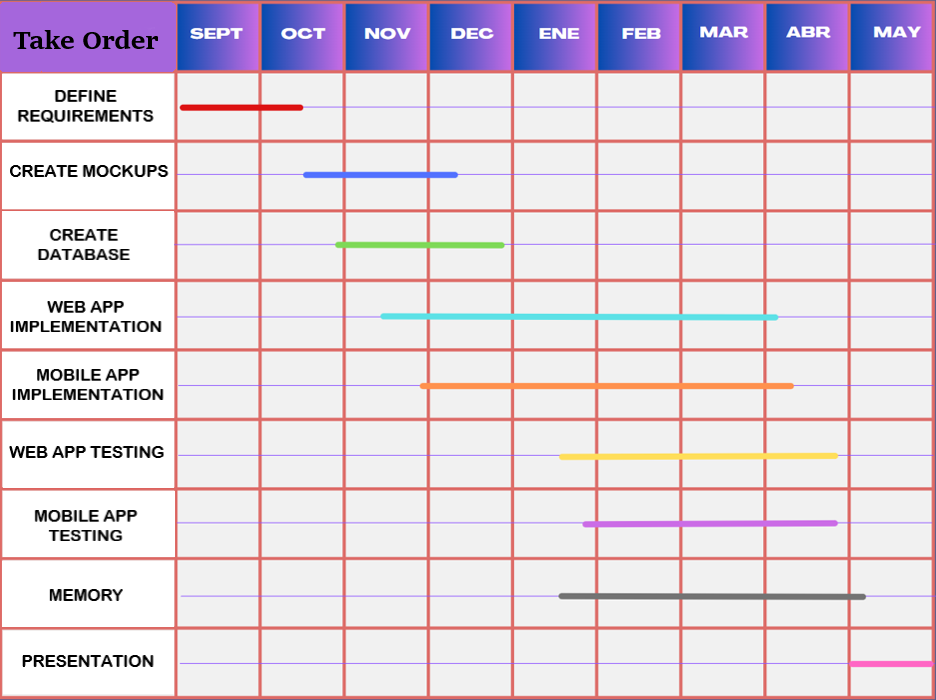
\includegraphics[width=15cm, height=11cm]{Imagenes/Figuras/Diagrama de Gantt (ingles).png}
\caption{Work plan}\label{fig:Diagrama de Gantt(ingles)}
\end{figure} 


\begin{figure}[h]
\centering
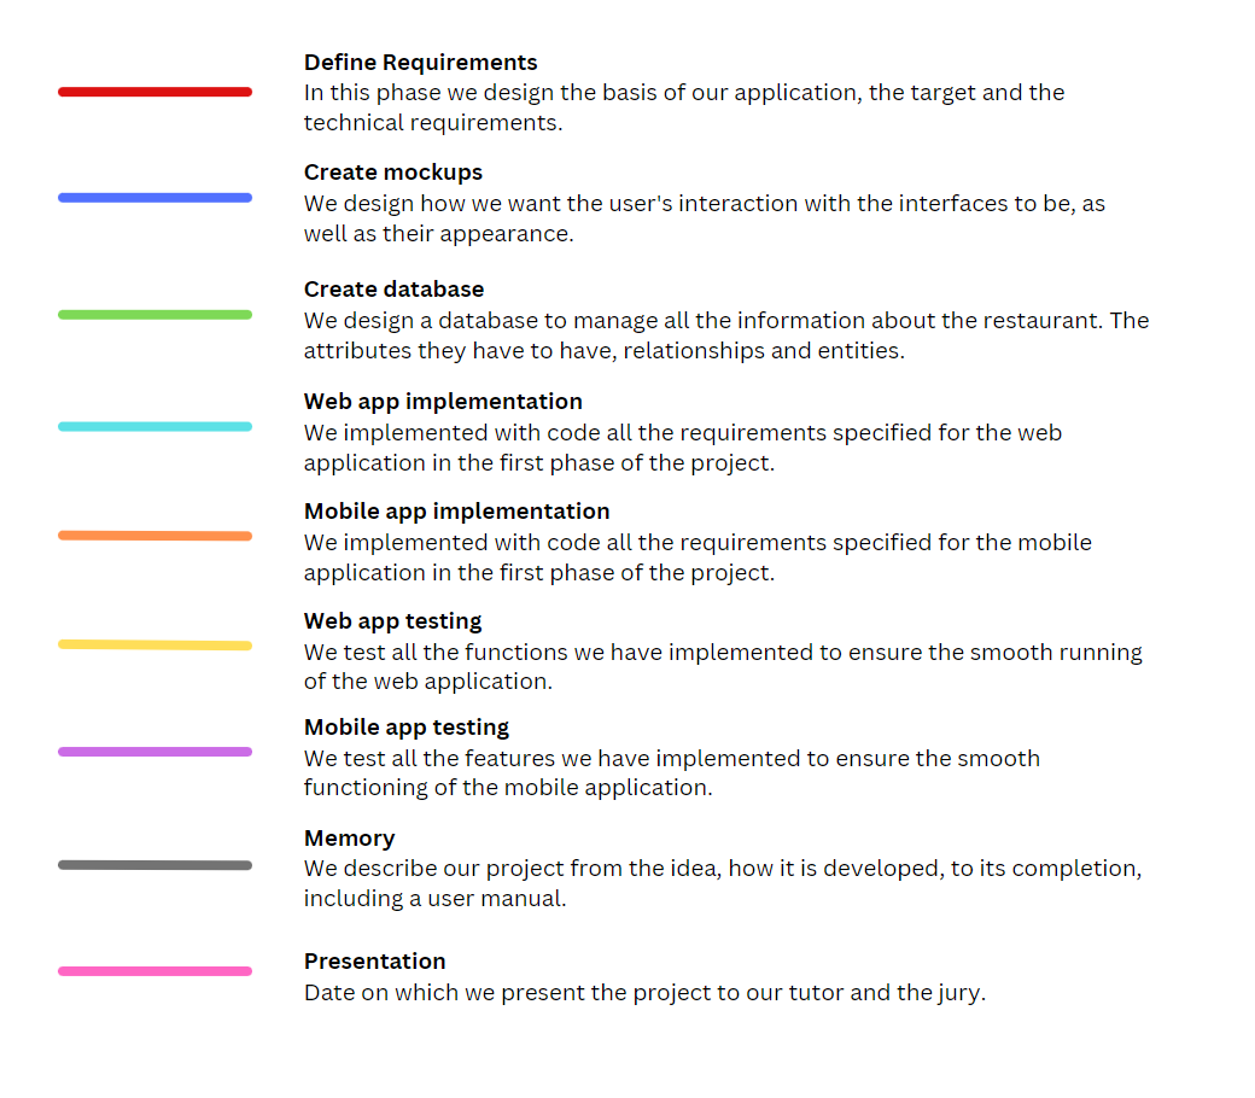
\includegraphics[width=15cm, height=12cm]{Imagenes/Figuras/leyenda Gantt (ingles).png}
\caption{Work plan legend}\label{fig:Leyenda diagrama de Gantt(ingles)}
\end{figure} 







